%v4.4
\subsection{Hadron Calorimeter (HCal)}\label{sec:expsetup_hcal}

\subsubsection{Description}

The Hadron Calorimeter (HCal) has been designed specifically to measure the recoil nucleon for the SBS experiments. Specifically for this experiment (and for $G_M^n$), HCal combined with the SBS (48D48) magnet provides identification of the recoil nucleon, as well as additional kinematic constraint and possibly timing information on the measured interaction.
Nucleon identification is illustrated on Fig.~\ref{fig:hcal_nuclimprint}. This figure shows the compared proton and neutron position distribution in HCal at the same electron kinematics. The proton distribution is being shifted upwards by about $1~\mathrm{m}$ compared to the neutron.

\begin{figure}[!h]
  \centering
    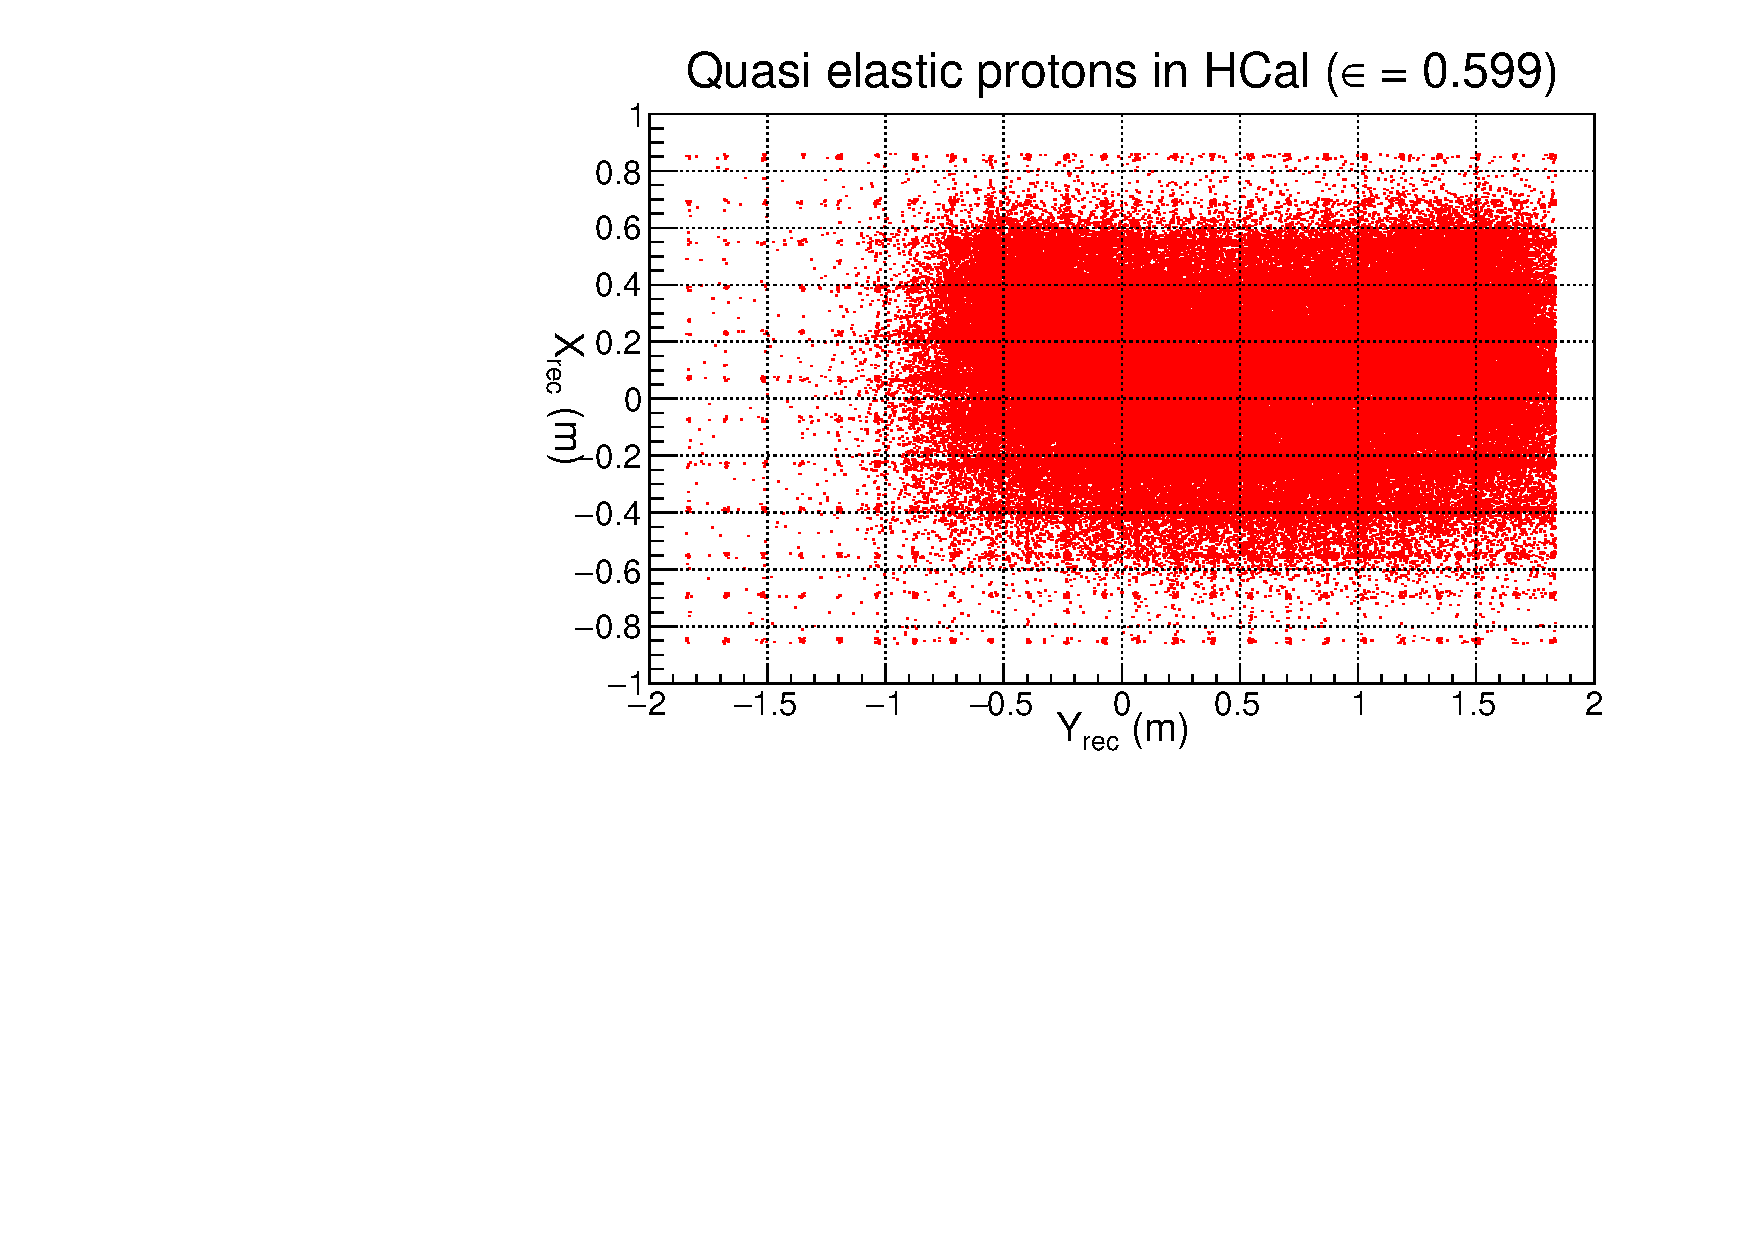
\includegraphics[angle=90,width=4cm]{Plots/HCal_p.pdf}
    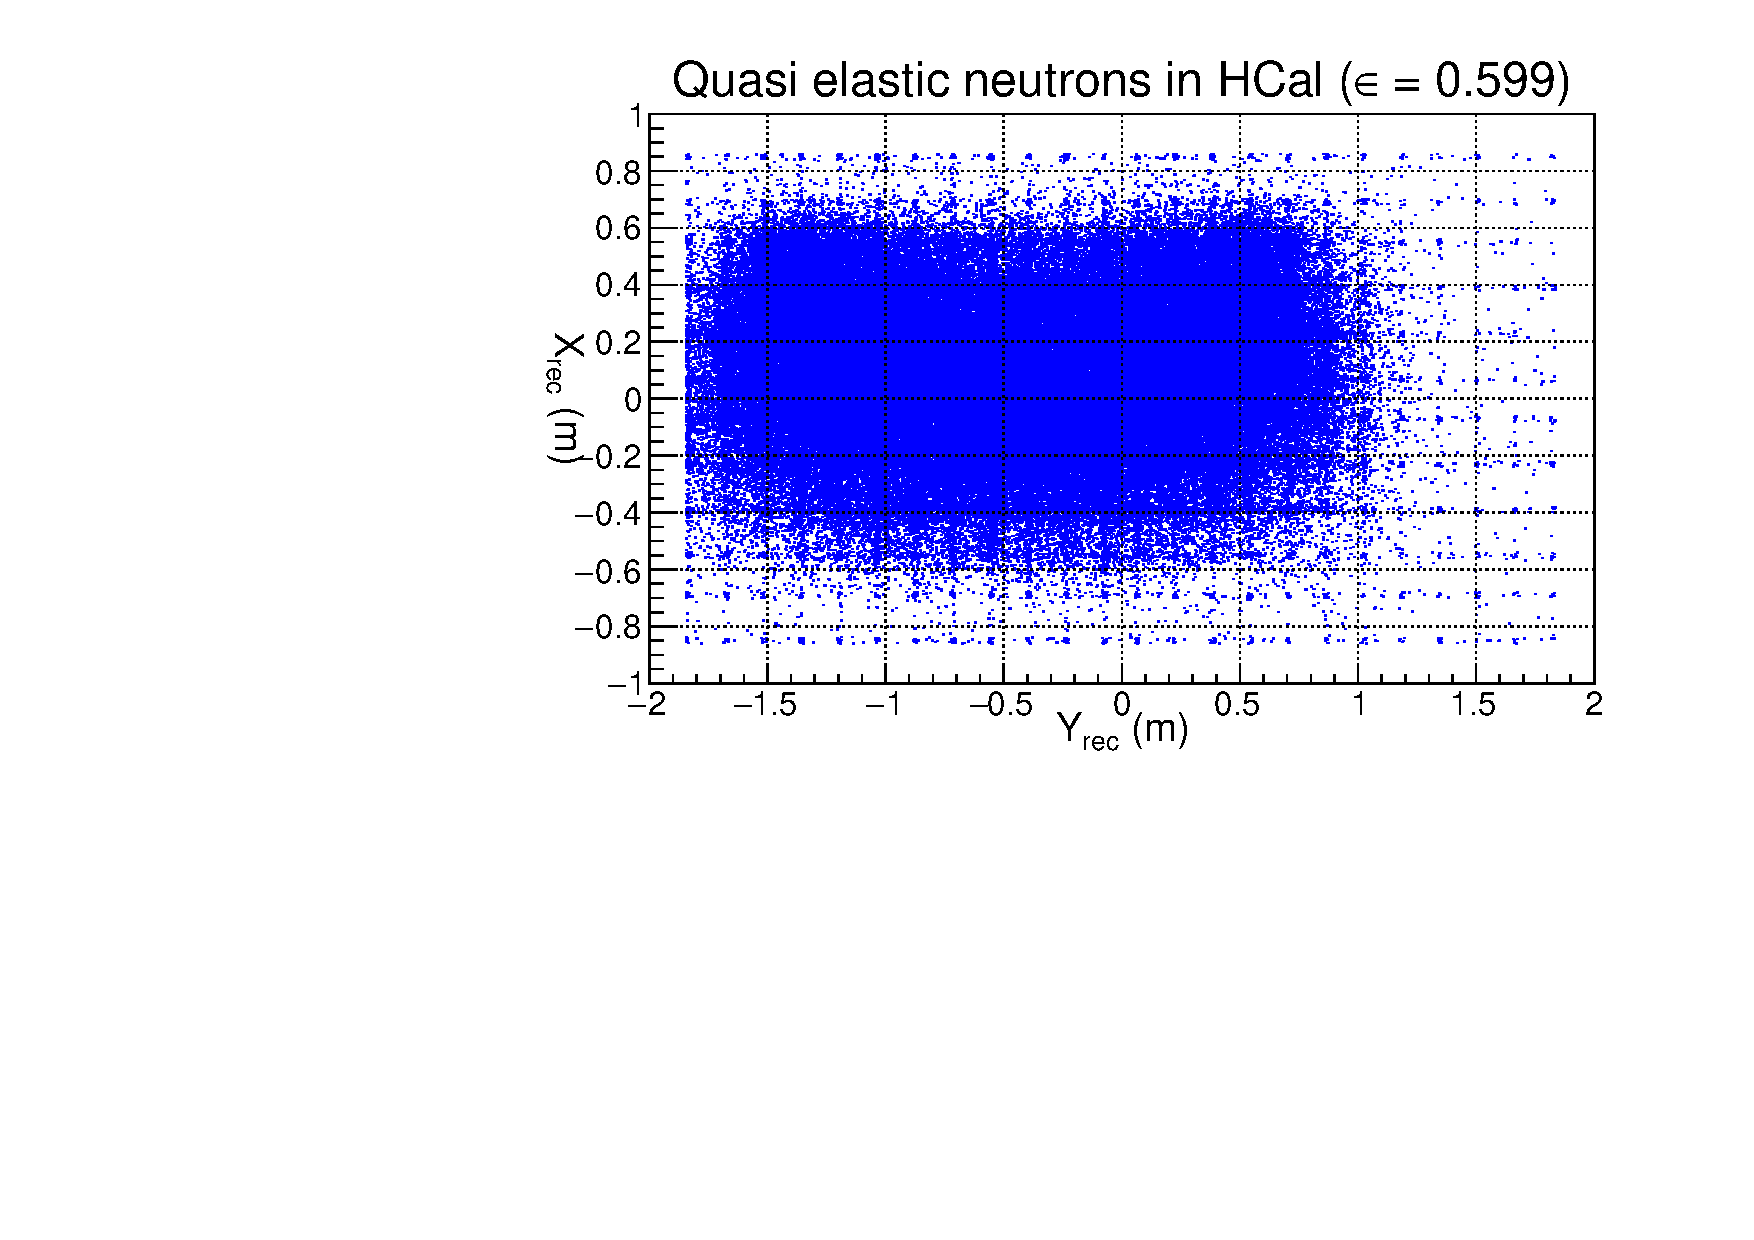
\includegraphics[angle=90,width=4cm]{Plots/HCal_n.pdf}
    \caption{Reconstructed HCal cluster from quasi-elastic events generated by G4SBS. The left distribution in red is for the proton, the right distribution in blue is for the neutron.}
    \label{fig:hcal_nuclimprint}
\end{figure}

The HCal (a CAD model of which is shown in Fig.~6)%\ref{fig:hcal_cad})
is composed of 288 modules arranged in an array of $12\, \times \, 24$.
%
\begin{figure}[!h]
  \centering
    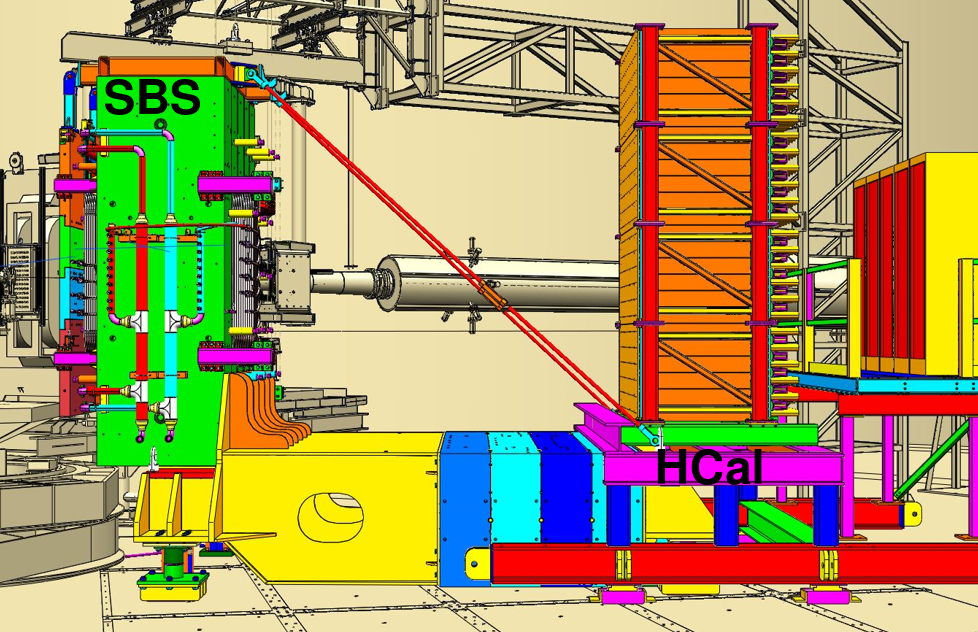
\includegraphics[width=10cm]{Plots/Wines_SBS_CAD_Fall2018.png}
    \caption{CAD representation of HCal (right) with the SBS magnet (left)}
    \label{fig:hcal_cad}
\end{figure}
%
In front of the full assembly is located a $3/4-\mathrm{inch}$ steel plate which serves two purposes:
%
\begin{itemize}
\item{initiate the hadronic shower to optimize the calorimeter response;}
\item{shield the modules from a fraction of the low energy secondaries;}
\end{itemize}
%
Each of these modules measures $6\,\times~6\,\mathrm{in}^2$ section, for $3~\mathrm{ft}$ length. They are composed of alternating tiles of scintillators and iron around a central light guide which collects the light generated in the scintillators by the hadronic shower, and guides it to the PMT at the end of the block.
Cosmic tests have determined that the average light yield for the HCal modules is around 5 photoelectrons per MeV deposited in the scintillator tiles.

The PMTs are read out with FADC250 which sample the PMT signal every 4 ns and allow to reconstruct the PMT pulse shape, and hence its timing.
They are also read out by TDCs which provide additional timing information.
Thanks to this, the timing resolution can be better than $1~\mathrm{ns}$, which cosmics tests (in progress) seem to confirm.

The energy resolution is intrinsically broad (see Fig.~\ref{fig:HCalRates} in Section~\ref{sec:simu}), due mostly to the small fraction of energy from the hadronic shower actually measured by the scintillator tiles ($\leq 0.1$ - refer yet again to Fig.~\ref{fig:HCalRates}).

%Note that the photoelectron statistics in the PMTs should not be a huge contributor to the resolution width. 
%\subsubsection{Parameters of the HCal}
\iffalse
The HCal angle and distance to the target will move from a kinematic to the other. At 8.5 m which is the largest distance for this experiment, the solid angle from the target is about 90 msr.
The matching between the electron in BigBite and the nucleon in HCal is about 90\% for the low $\epsilon$ kinematic.
For the high $\epsilon$ kinematic, HCal has to be brought closer to the target because the nucleon imprint is larger (Fig.~\ref{fig:hcal_nuclimprint2}).
%\iffalse
%
\begin{figure}[!h]
  \begin{center}
    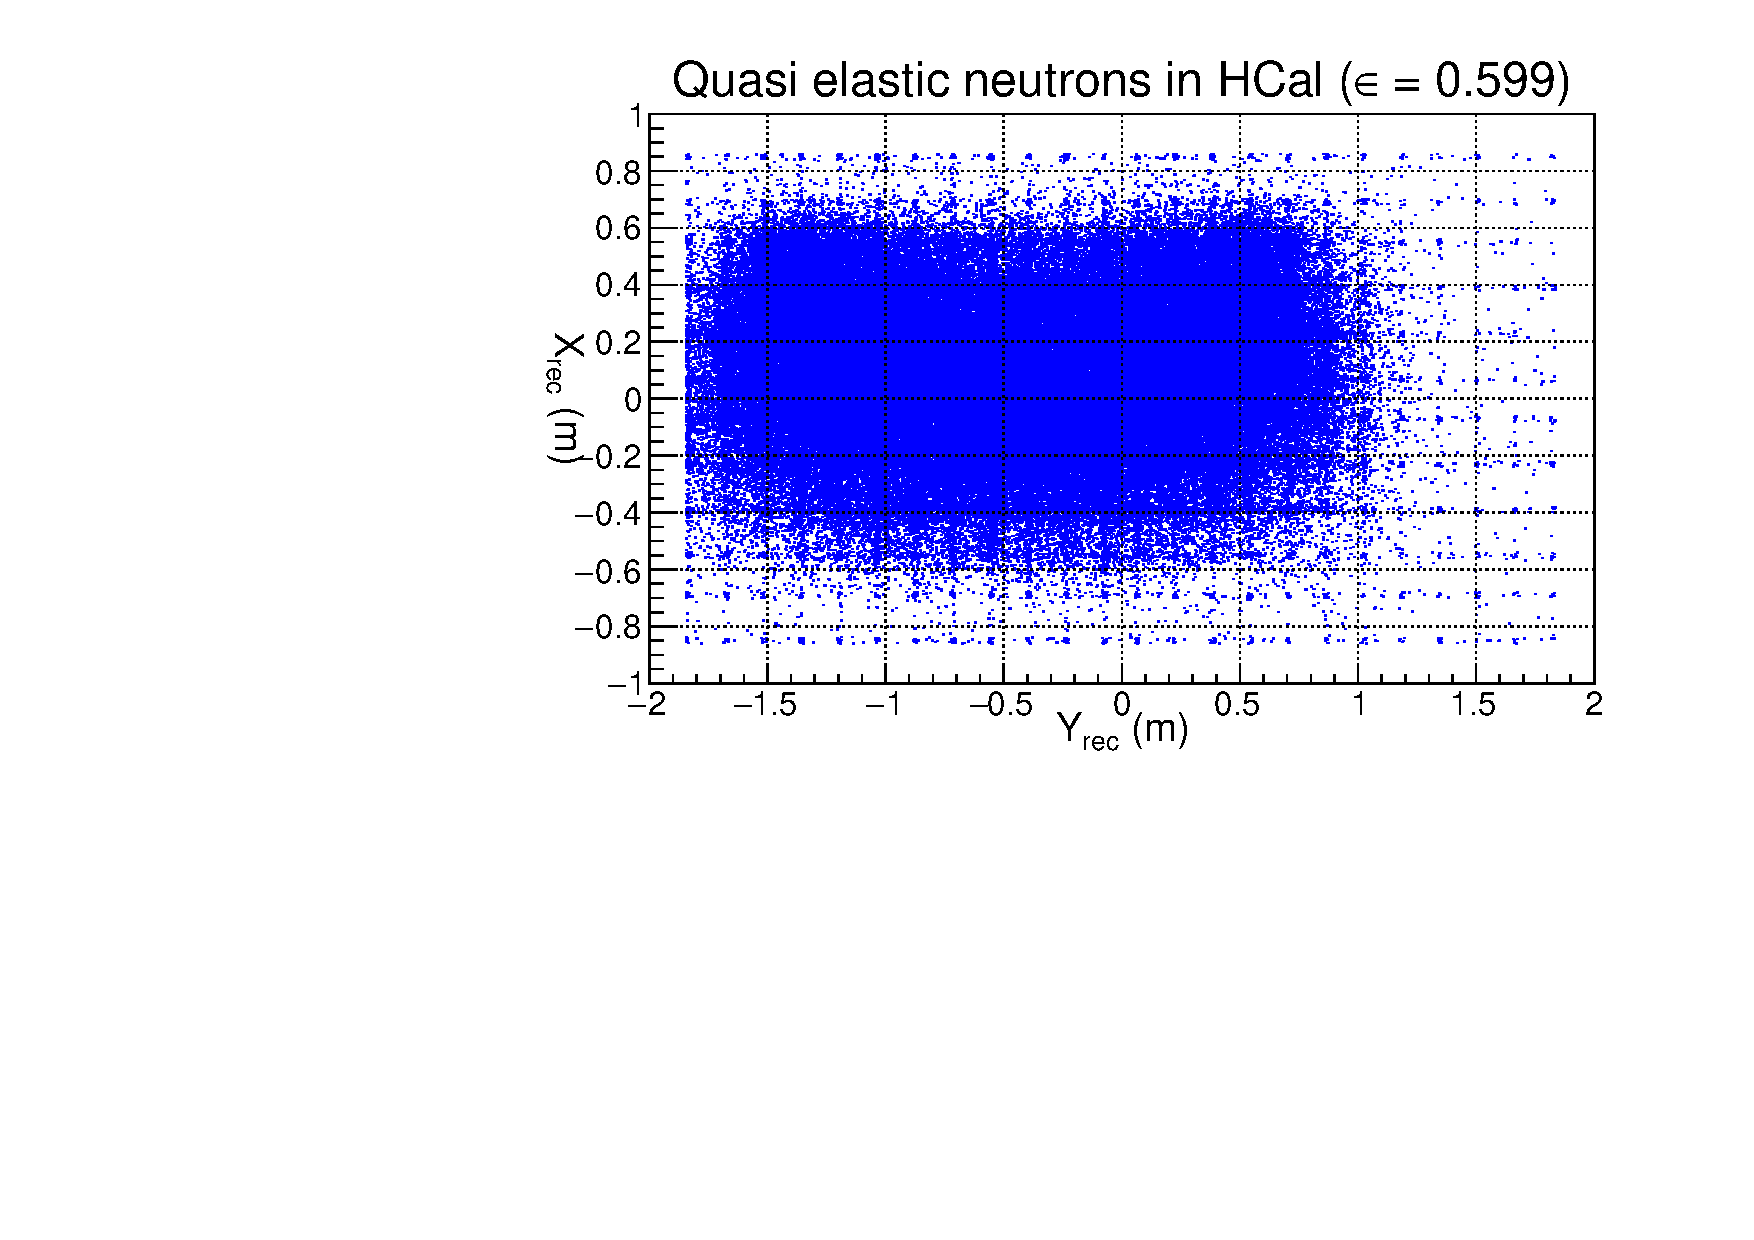
\includegraphics[angle=90,width=4cm]{Plots/HCal_n.pdf}
    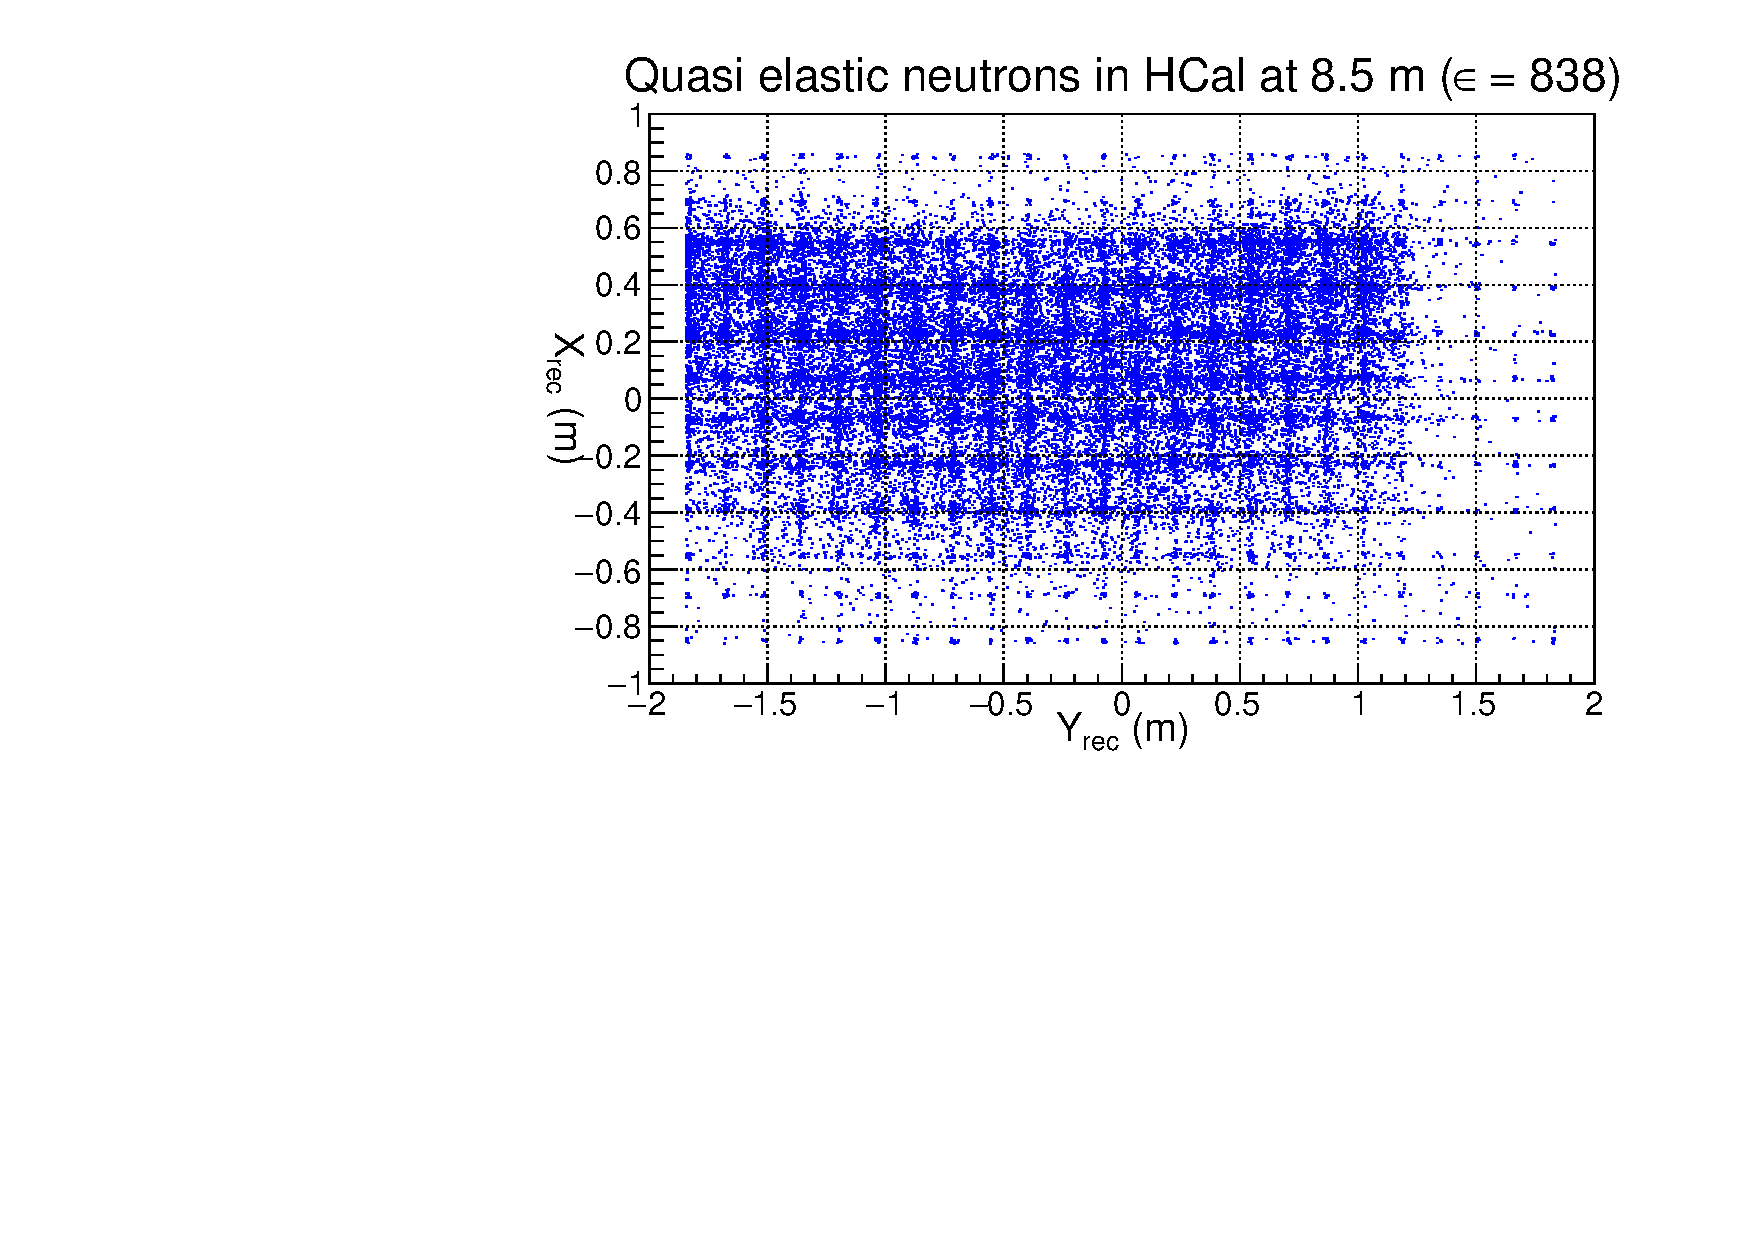
\includegraphics[angle=90,width=4cm]{Plots/HCal_n_he.pdf}
    \caption{Reconstructed HCal cluster from quasi-elastic events generated by G4SBS. The left distribution is for the neutron at the low $\epsilon$ kinematic, the right distribution is for the neutron at the high $\epsilon$ kinematic, and the same distance from the target.}
    \label{fig:hcal_nuclimprint2}
  \end{center}
\end{figure}
%
\fi

\subsubsection{Discussion on HCal efficiency}

A crucial parameter of this experiment is the hadron calorimeter efficiency, which is expected to be slightly different for protons and neutrons, and more importantly the efficiency stability. %provides hadron identification.

\paragraph{Experimental evaluation of HCal efficiency}

The calorimeter efficiency will be measured by using "elastic" reactions H$(e,e’)p$, H$(\gamma,\pi^+)n$
and more with D$(\gamma,\pi^+)n$ and D$(\gamma,\pi^-)p$ single pion production.
Fig.~\ref{fig:Nproj}~{\bf(a)} shows the projected proton position from H$(e,e’)p$, 
Fig.~\ref{fig:Nproj}~{\bf(b)} shows the projected proton position from H$(\gamma,\pi^+)n$.
%
\begin{figure}[!h]
  \centering
  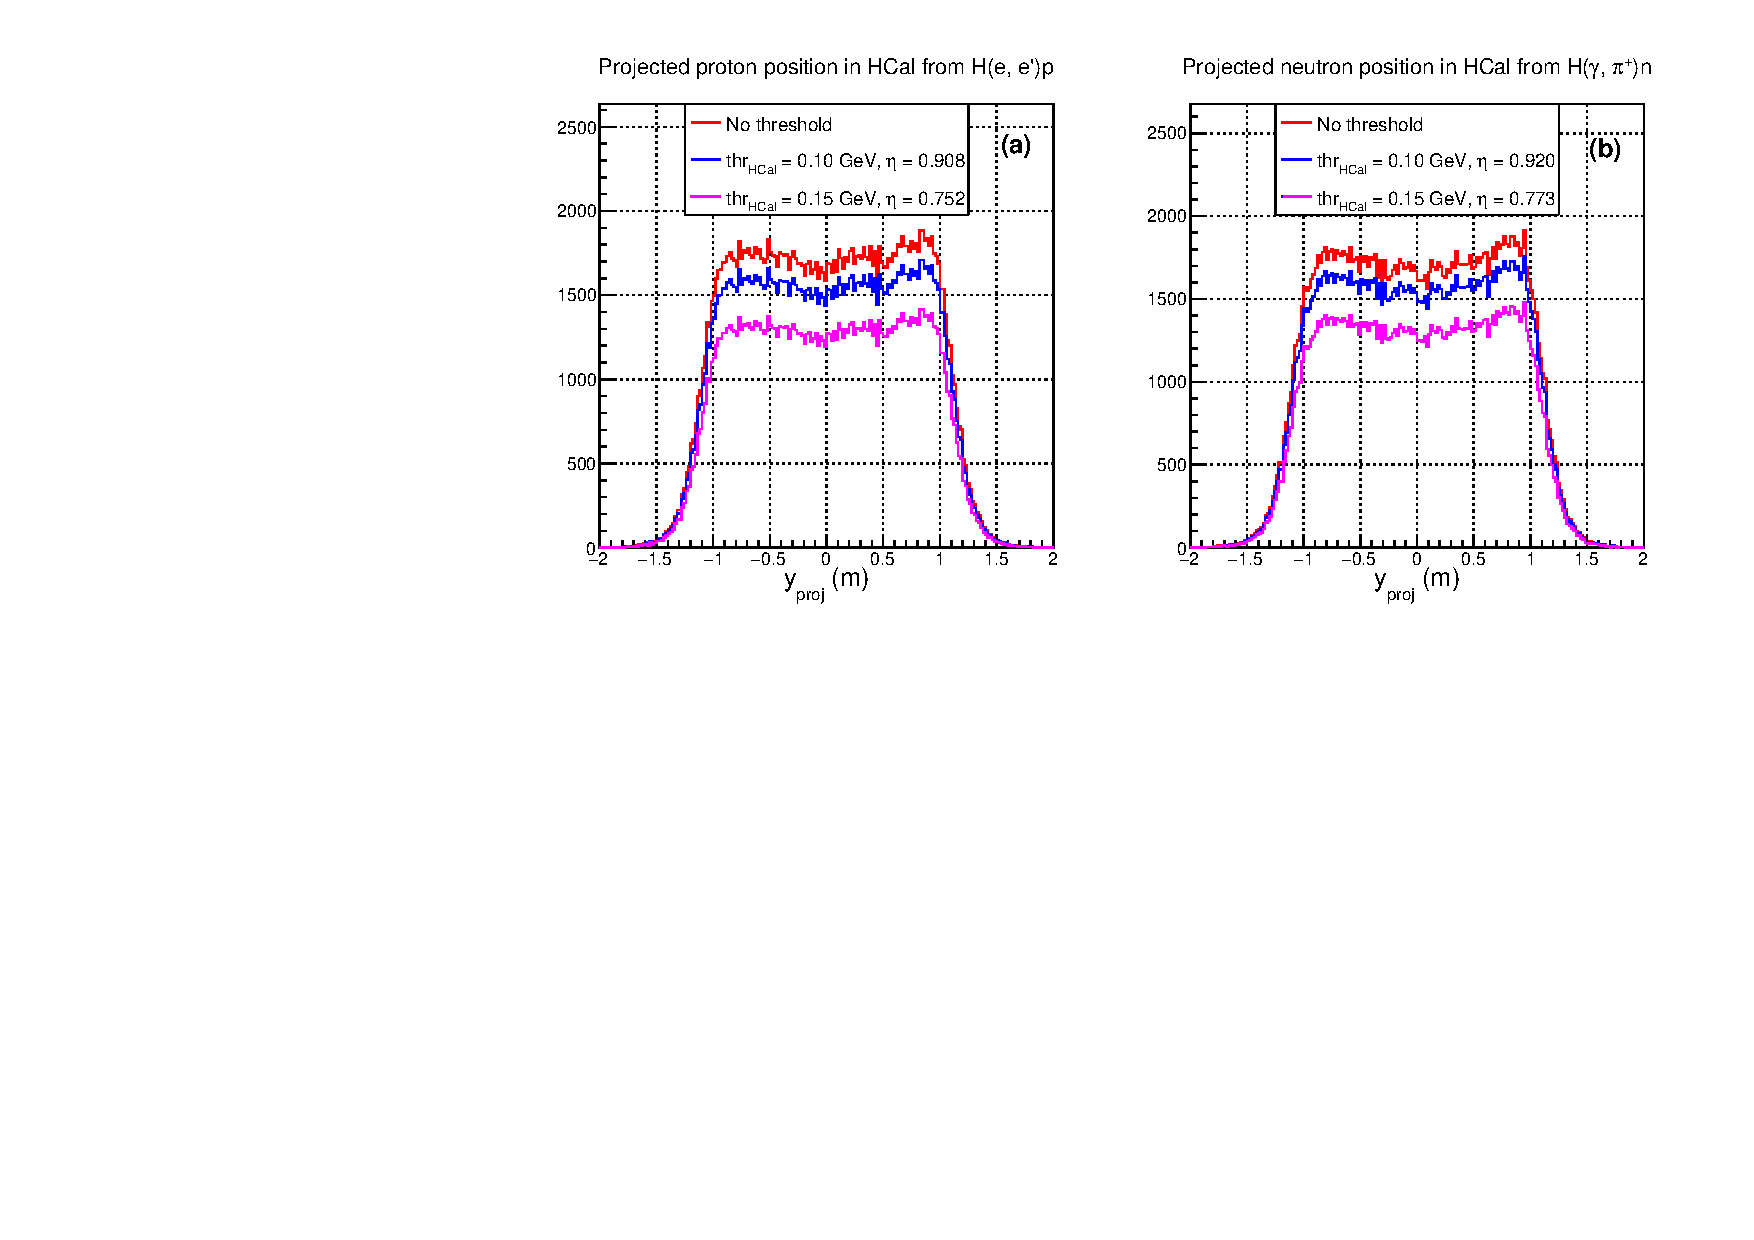
\includegraphics[width=12cm]{Answers_Readers/ProtVsNeut_CalibYproj.pdf}
  \caption{Projected position in HCal in for the protons in H$(e,e’)p$~{\bf(a)} and the neutrons in H$(\gamma,\pi^+)n$~{\bf(b)}. On both panels, red distributions show the projected distribution for $p$, $n$, not detected; blue distributions show the distribution for $p$, $n$ detected with a 0.1 GeV threshold; magenta distributions show the distribution for $p$, $n$ detected with a 0.15 GeV threshold.}
  \label{fig:Nproj}
\end{figure}
%
In each case, the trigger will not use the nucleon detector information.
Analysis will use the amplitude distribution in the same way as done on  Fig.~\ref{fig:Neff} with the red distributions.
Blue distributions on Fig.~\ref{fig:Nproj} show the expected Y distribution applying a 0.10 GeV threshold on HCal;
Magenta distributions on Fig.~\ref{fig:Nproj} show the expected Y distribution applying a 0.15 GeV threshold on HCal.
As reported in the E12-09-019 GMn proposal\footnote{https://www.jlab.org/exp\_prog/proposals/09/PR12-09-019.pdf} on Table~8, the expected recorded statistics for H$(\gamma,\pi^+)n$ are of the order of 4000 events, which will represent a relative 1.5\% uncertainty on the neutron efficiency. The recorded statistics for H$(e,e’)p$ are of the order of 82000 events, which will represent a relative 0.3\% uncertainty on the proton efficiency.\\

\paragraph{Impact of efficiency ratio on the neutron / proton yields ratio}

{\hskip 0.7cm}We want to evaluate the impact of the ratio of hadron efficiencies,\\
$R_{\eta_{n/p}} = \eta_n/\eta_p$
on the ratio of neutrons to proton yields $R_{n/p} = N_{en}/N_{ep}$.

To obtain the ``true'' ratio of neutrons to proton yields $R_{n/p}$ from the recorded ``raw''
ratio of neutrons to proton yields $R_{n/p, raw}$,
this ratio needs to be corrected by $R_{n/p}$.
%
\begin{equation}
  R_{n/p} = R_{n/p, raw}/R_{\eta_{n/p}}
\end{equation}
%
Hence, the uncertainty, $\Delta R_{n/p}$ of $R_{n/p}$ could be expressed as:
%
\begin{equation}
  \Delta R_{n/p}/R_{n/p} = \Delta R_{\eta_{n/p}}/R_{\eta_{n/p}}.
\end{equation}
%
To evaluate the uncertainty of $R_{\eta_{n/p}} = \eta_p/\eta_n$,
we need to account for the strong correlation between $\eta_p$ and $\eta_n$, $\rho_{\eta_{n/p}}$. 
We can define the covariance between the uncertainties $\Delta \eta_p$ and $\Delta \eta_n$,
$\sigma_{\eta_{n/p}} = \rho_{\eta_{n/p}} \Delta \eta_{n} \Delta \eta_{p}$ \footnote{https://en.wikipedia.org/wiki/Covariance\_and\_correlation}.

According to\footnote{https://www.sagepub.com/upm-data/6427\_Chapter\_4\_\_Lee\_(Analyzing)\_I\_PDF\_6.pdf}, we can write the uncertainty on the ratio efficiencies:
%\footnote{line~5 of table in https://en.wikipedia.org/wiki/Propagation\_of\_uncertainty\#Example\_formulae}

%
%\begin{equation}
\begin{align}
  \frac{\Delta R_{\eta_{n/p}}}{R_{\eta_{n/p}}} &= \sqrt{ \left( \frac{\Delta \eta_{n}}{\eta_{n}} \right)^2
    + \left( \frac{\Delta \eta_{p}}{\eta_{p}} \right)^2
    - 2 \frac{\sigma_{\eta_{n/p}}}{\eta_{n}\eta_{p}} }
  \\
  &= \sqrt{ \left( \frac{\Delta \eta_{n}}{\eta_{n}} \right)^2
    + \left( \frac{\Delta \eta_{p}}{\eta_{p}} \right)^2
    - 2 \frac{\rho_{\eta_{n/p}} \Delta\eta_{n} \Delta\eta_{p}}{\eta_{n}\eta_{p}} }
  \label{eq:uncert_exact}
  %\end{equation}
\end{align}
%
\begin{figure}[!h]
  \centering
  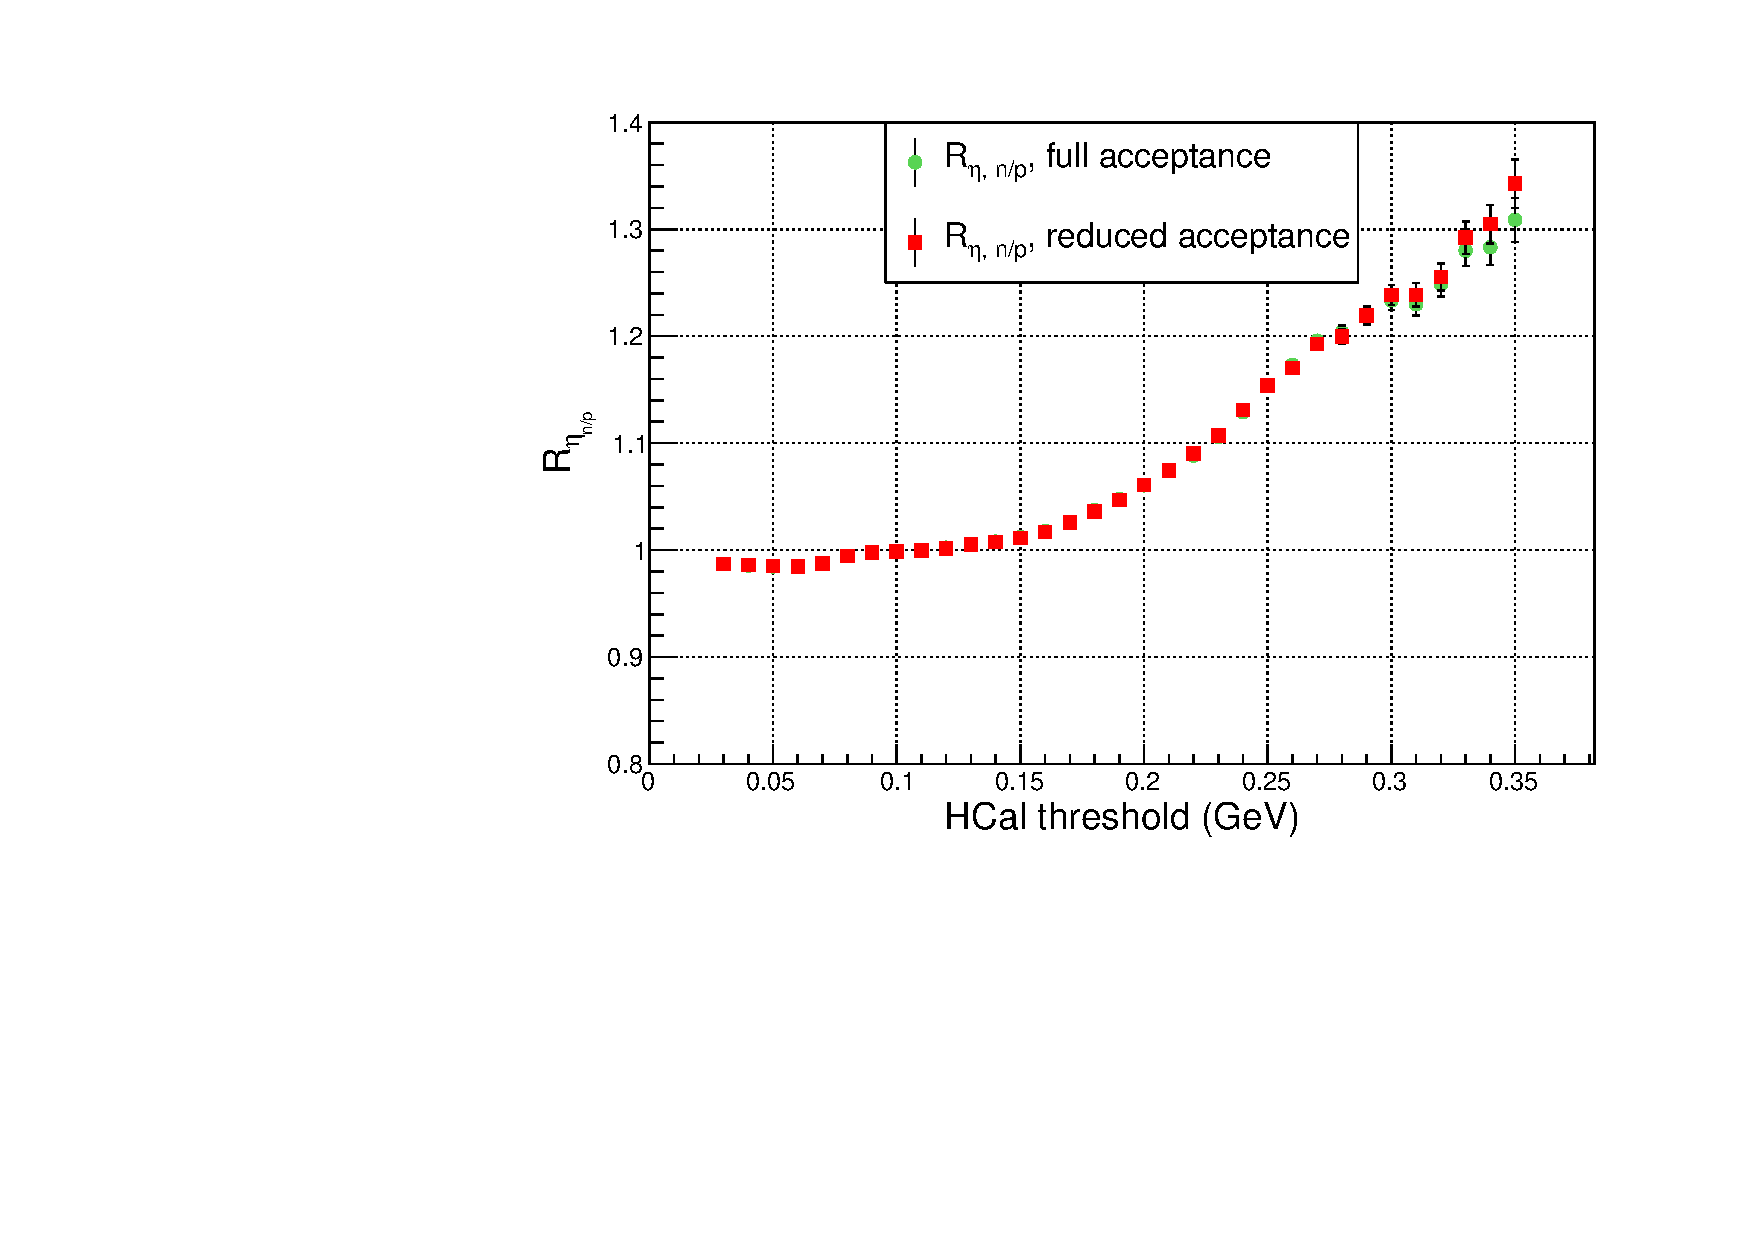
\includegraphics[width=7cm]{Answers_Readers/Reta_np_fthr_errs.pdf}
  \caption{Neutron/proton efficiency ratio $R_{\eta_{n/p}}$ as a function of the calorimeter threshold, for our quasi-elastic sample. The error bars represent the uncertainty from the calibration measurements discussed earlier. The green represents $R_{\eta_{n/p}}$ on the full acceptance, the red represents $R_{\eta_{n/p}}$ on a reduced acceptance.
    % The discrepancy between the two (blue) is about 0.1\% below a threshold of 0.15 GeV.%, but becomes about 0.5\% between 0.15 and 0.3 GeV, up to 1\% beyond 0.3 GeV}
  }
  \label{fig:Reta_np}
\end{figure}
%
$\Delta\eta_{p}$ and $\Delta\eta_{n}$ are the uncertainties from the calibration measurements described above.%on the Monday write up. %$\sigma_{\eta-n/p}$. Fig~\ref{fig:Reta_np}.
The correlation between the variations of the proton and neutron efficiencies $\rho_{\eta_{n/p}}$, depends on the cause of the variations.
In the case of the efficiency calibrations runs, discussed in the Monday write-up,
the uncertainties of the efficiencies are due to the statistic of the collected events. 
In such a case, $\rho_{\eta_{n/p}} = 0$.
However, in the case of the detector instability, $\rho_{\eta_{n/p}} \sim 1$ (see again Fig.~\ref{fig:Reta_np}).

With the statistics projected for the calibration runs: $\eta_p \pm \Delta\eta_{p} = 0.915 \pm 0.003$ and $\eta_n \pm \Delta\eta_{n} = 0.924 \pm 0.014$.
Applying these values to Eq.~\ref{eq:uncert_exact}, %, and considering $R_{\eta_{n/p}} = 0.991$,
the relative uncertainty on the absolute value of the hadron efficiency ratio becomes:
%
\begin{equation}
  \Delta R_{\eta_{n/p}}/R_{\eta_{n/p}} = 1.6\%.
\end{equation}
%
Considering $R_{\eta_{n/p}} = 0.991$ from Fig.~\ref{fig:Reta_np}, $\Delta R_{n/p}/R_{n/p} = 0.016$. 
This would add up to the total systematic uncertainty of $R_{n/p}$ to 1.9\% for the low $\epsilon$ kinematic and to 1.6\% for the high $\epsilon$ kinematic.\\

However, %as it was demonstrated in Tuesday's write-up,
the measurement of the Rosenbluth slope, $S^n = \sigma_L/\sigma_T$, is unaffected by the uncertainty of the absolute value of the efficiency ratio $R_{\eta_{n/p}}$.
$R_{\eta_{n/p}}$ will be cancelled in the the determination of the neutron Rosenbluth slope $S^n$, 
{\it as long as we control the stability of $R_{\eta_{n/p}}$ over the few days of the measurement}.

\paragraph{Impact of efficiency stability on the Rosenbluth slope meansurement}

The specific value of the hadron calorimeter efficiency does not impact the quality of the experimental result.
However, the stability of the efficiency ratio is essential.

Let us evaluate in detail the influence of the hadron efficiencies, $\eta_n$ and $\eta_p$, on the experimental result.
%and proton efficiency $R_{\eta_{n/p}} = \eta_n/\eta_p$ on the measurement of $R_{corrected} = R_{n/p} \times f_{corr}$ and $S^n$.
The $S^n$ result is sensitive only to the ratio of neutron efficiency to proton efficiency, $R_{\eta} = \eta_n/\eta_p$.
Such a ratio is very stable because the nucleon momenta are the same by definition of the Rosenbluth method.   
We have a plan to monitor the stability of this ratio in our experimental data.

Our primary experimental observable is the ratio of yields $R_{n/p} = N_{en}/N_{ep}$.
In this experiment, the parameter of interest is $A = [R_{n/p, \epsilon-1}/R_{n/p, \epsilon-2}]\times[R_{\eta, epsilon-1}/R_{\eta, epsilon-2}]$.

As we wrote in our proposal, pages 12 and 13, and under the assumption that the reduced cross section $\sigma_R$ is linear in $\epsilon$,
the neutron Rosenbluth slope $S^n$ can be obtained as:
%
\begin{equation}
  S^n = \frac{A-1}{\Delta\epsilon} + S^p = (\frac{R_{n/p, \epsilon-1}}{R_{n/p, \epsilon-2}}\times \frac{R_{\eta, epsilon-1}}{R_{\eta, epsilon-2}}-1)/\Delta\epsilon + S^p
  \label{eq:Sn}
\end{equation}
%
As it is easy to see from the formula above, the efficiency impact cancels out in $S^n$ if the efficiency ratio is stable.

The procedure to evaluate the hadron detector efficiency was described above.
The result will be fitted by a few parameter functions, and the ratio of efficiency $R_{\eta}$ is characterized by those parameters as well as the threshold.
This study will be performed for all modules of HCal used in the experiment.
After the data collection, we will repeat this study with the recorded data for each kinematic.
Based on projected statistics of a few million events, the accuracy of $R_{\eta}$ will be better than 0.1\%.
With such an accuracy, we will monitor the stability of $R_{\eta}$.
This corresponds to the uncertainty in $S^n$, using the formula above, of 0.004, with our $\Delta \epsilon = 0.24$. 

Additional analysis of the efficiency ratio is presented on Fig~\ref{fig:Reta_np}.
This analysis focused on absolute value of efficiency ratio, for which we expect 1\% statistical level.
To monitor the stability, we will have hundreds of times more statistics.
%
\begin{figure}[!h]
  \centering
  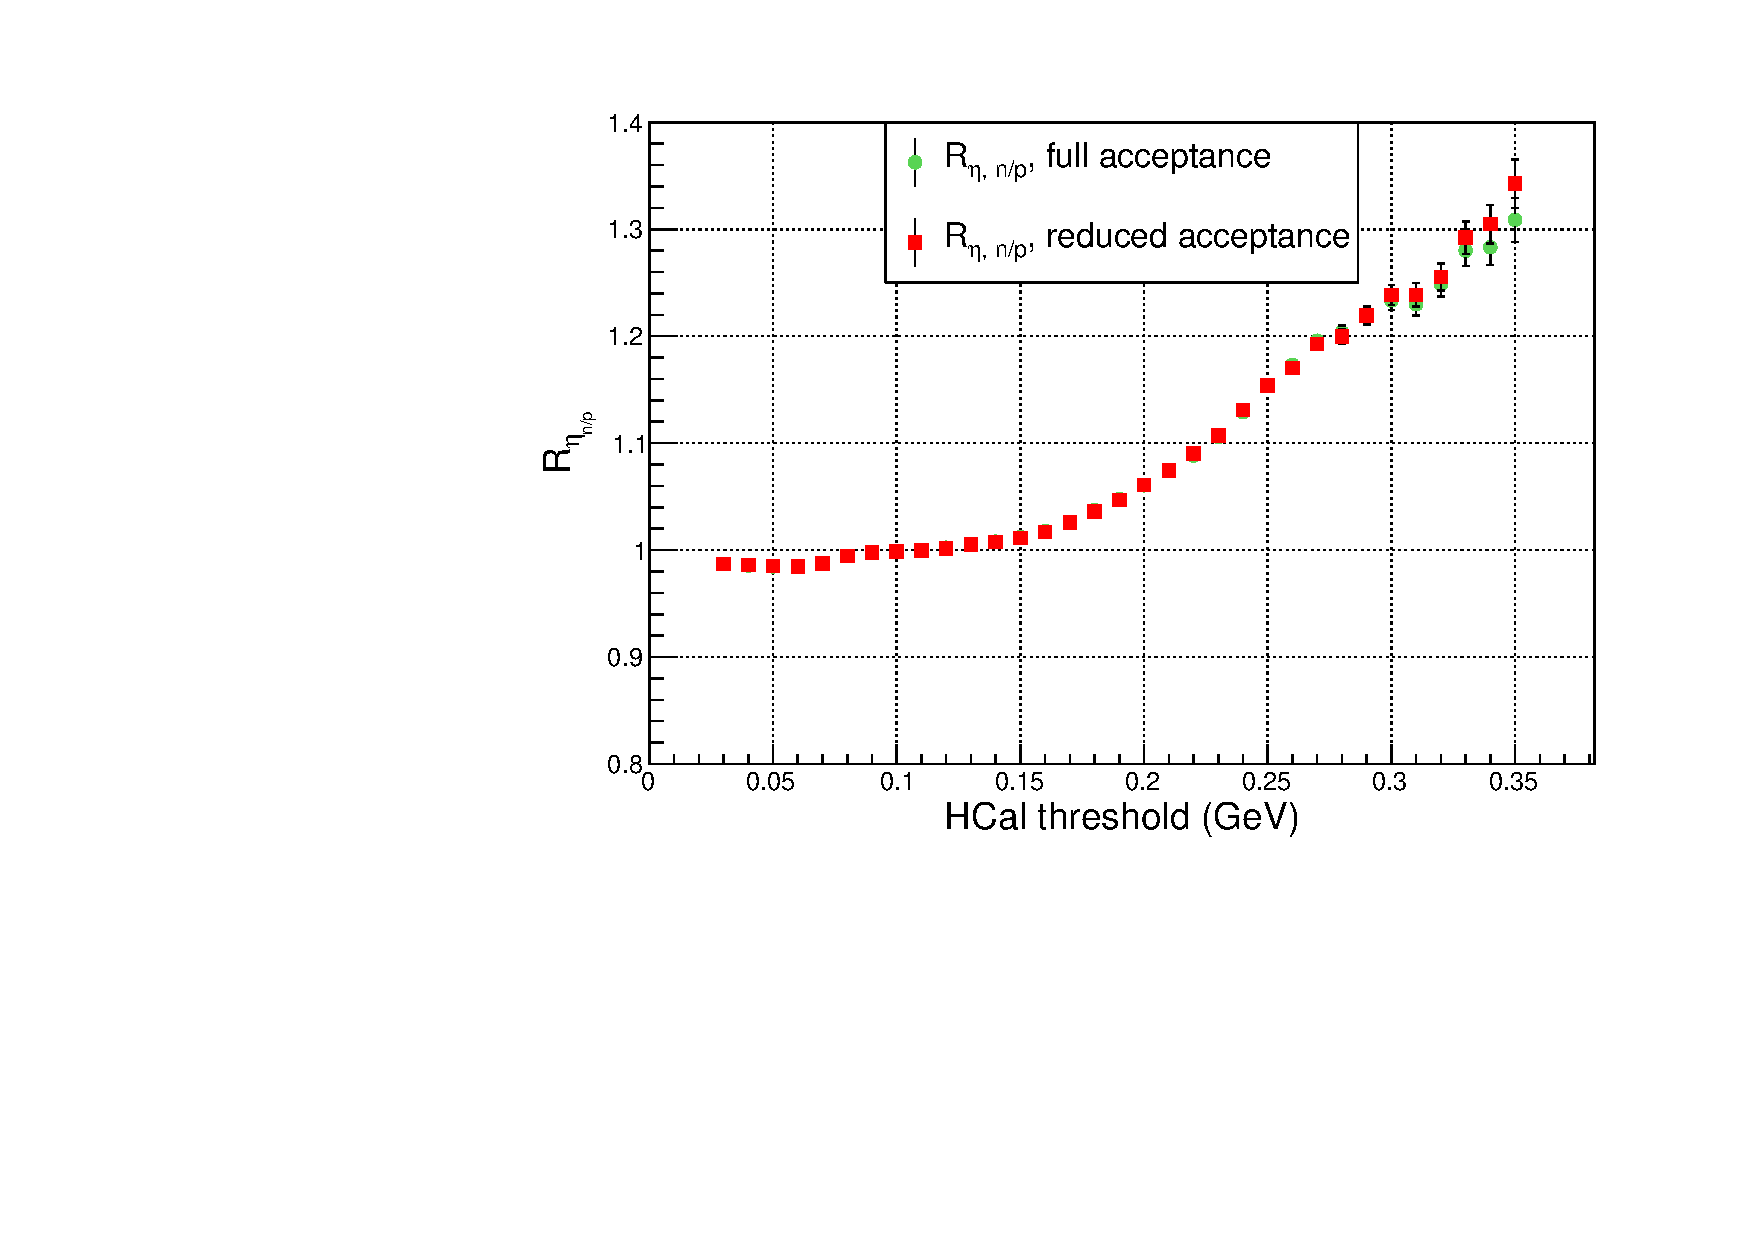
\includegraphics[width=7cm]{Answers_Readers/Reta_np_fthr_errs.pdf}
  \caption{Neutron/proton efficiency ratio $R_{\eta_{n/p}}$ as a function of the calorimeter threshold, for our quasi-elastic sample. The error bars represent the uncertainty from the calibration measurements discussed earlier. The green represents $R_{\eta_{n/p}}$ on the full acceptance, the red represents $R_{\eta_{n/p}}$ on a reduced acceptance. %The discrepancy between the two (blue) is about 0.1\% below a threshold of 0.15 GeV.%, but becomes about 0.5\% between 0.15 and 0.3 GeV, up to 1\% beyond 0.3 GeV}
            }
  \label{fig:Reta_np}
\end{figure}
%

\paragraph{Efficiency stability due to the detector parameters drift}

As we know, the stability of the hadron detector efficiency is critical for a successful measurement.
The instability of the efficiency $\eta$ over time is mainly due to the drift of the PMTs signals and the related electronics.
Such an amplitude drift is typically of 1-2\% over a few days.
It will be better for our detector thanks to the LED calibration system.

We expect to use a threshold $A_{thr}$ = 100 MeV (see plots of amplitude spectrum in the Monday write-up).
Using the graph of the nucleon detection efficiency as a function of the threshold $A_{thr}$ on Fig.~\ref{fig:eta_N},
we find that, in the region $A_{thr} = 90 - 110$~MeV, the efficiency is:
%
\begin{equation}
  \eta = 0.92 - 0.18 \times \frac{A[{\rm MeV}]-100}{100}
\end{equation}
%
A one percent variation of $A_{thr}$ leads to 0.2\% variation of efficiency.
%
\begin{figure}[!h]
  \centering
  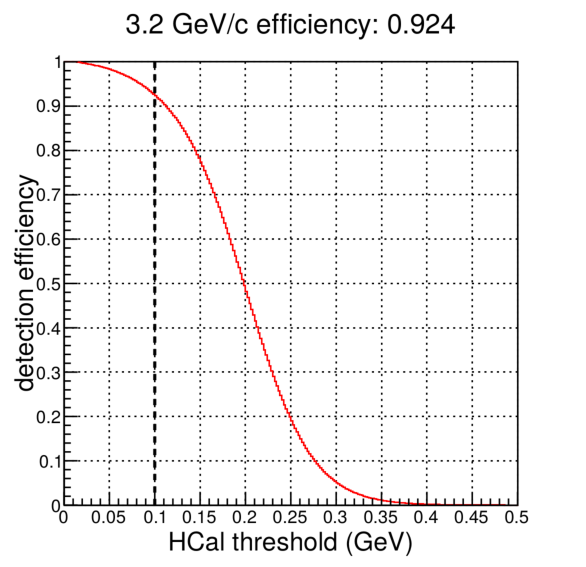
\includegraphics[width=7cm]{Answers_Readers/Neff_fThr.pdf}
  \caption{Nucleon detection efficiency vs the calorimeter threshold $A_{thr}$.}
  \label{fig:eta_N}
\end{figure}
%

Turning now to the ratio of efficiencies, we plot it as a function of the threshold on Fig.~\ref{fig:Reta_np}.
We find that, in the region $A_{thr} = 90 - 110$~MeV, the ratio of efficiencies is:
%
\begin{equation}
  R_{\eta_{n/p}} = \frac{\eta_n}{\eta_p} = 0.998 + 0.011 \times \frac{A[{\rm MeV}]-100}{100}.
\end{equation}
%
Using the estimate for a PMT-based system instability of 1-2\%, which means that $A_{thr}$ is stable to 1-2 MeV,
the ratio of efficiencies $R_{\eta_{n/p}} = \frac{\eta_n}{\eta_p}$ is found to be stable to 0.022\%.

The run plan of the GMn experiment (E12-09-019), which will run next summer,
has a provision of running on the hydrogen target multiple times with different fields in the SBS dipole,
allowing the study of the stability of individual modules of HCal.
